\subsection{Wealth Formal Model} \label{wealth-formal-model}
Knowledge graphs follow Resource Description Framework (RDF)~\cite{w3crdf} as a means of data organization. Without loss of generality of how the form of the URIs is, data is stored in the form of triple \((s, p, o)\); a combination of a subject \(s\), a predicate \(p\), and an object \(o\) which can be visualized as nodes and directed-arc diagrams. For example, the statement "William Shakespeare's notable work is Romeo and Juliet" in human-readable URIs is mapped to the triple (\textit{WilliamShakespeare}, \textit{notableWork}, \textit{RomeoAndJuliet}). Likewise, the statement in Wikidata, which uses ID-based URIs, is mapped to (\textit{Q692}, \textit{P800}, \textit{Q83186}).

There are 2 kinds of nodes: IRIs and literals. A triple is in the form of \((s, p, o) \in I \times I \times (I \cup L) \) where \(I\) is the node with type IRI and \(L\) is the node with type literal. A knowledge graph is a finite set of triples \((s, p, o)\).

% \subsubsection{Class}
% In this study, we re-use the class model defined by Ramadizsa et al. (2023). A class is a group of entities that are the subject of the study. \textit{Human}, \textit{film}, and \textit{taxon} are some examples of class. In general, entity \(s\) is an instance of class \(C\) is expressed by the triple (\(s\), \textit{instanceOf}, \(C\)) or (\(s\), \textit{type}, \(C\)). We can get a more narrow class inside the defined class by specifying additional conditions, each consisting of a particular property and value associated with it. Example of such conditions for human class is \textit{gender} with associated value \textit{male}, while example for a country would be \textit{continent} with value \textit{Asia}. For instance, the class of human with gender male that lived during English Renaissance is queried using (\(?s\), \{(\(?s\), \textit{instanceOf}, \textit{human}), (\(?s\), \textit{gender}, \textit{male}), (\(?s\), \textit{timePeriod}, \textit{EnglishRenaissance})\}).

\subsubsection{Entity-Level Wealth: Knowledge Wealth Type and Definition}

Let \(e \in I\) be an entity in a knowledge graph \(G\). We quantify the wealth of entity \(e\) in \(G\) as the amount of information about \(e\) available in \(G\). Thus, we define the knowledge wealth of an entity as the number of properties associated/linked to it. For example, the wealth of \textit{William Shakespeare} (\textit{Q692}) in Wikidata counts all triples describing \textit{Q692} in Wikidata, including those detailing his family, occupation, image, and so on.

As motivated in \Cref{introduction}, there are three key dimensions to consider when alculating the knowledge wealth of an entity: (1) wealth based on the (non-)uniqueness or multiplicity of individual property; (2) wealth based on type of property; and (3) wealth based on the direction of the link. We denote the knowledge wealth of an entity \(e\) in graph \(G\) using the general form:
\[
    W_{mult,[prop],[dir]}(e,G)
\]
where:
\[
    mult \in  \{bag, set\}
\]
\[
    prop \subseteq  \{obj, ltr, id\}
\]
\[
    dir \subseteq  \{out, in\}
\]
This formalization provides a flexible and expressive way to define and compute knowledge wealth under different configurations.

\begin{figure}[!h]
    \centering
    \begin{subfigure}[b]{0.3\textwidth}
        \centering
        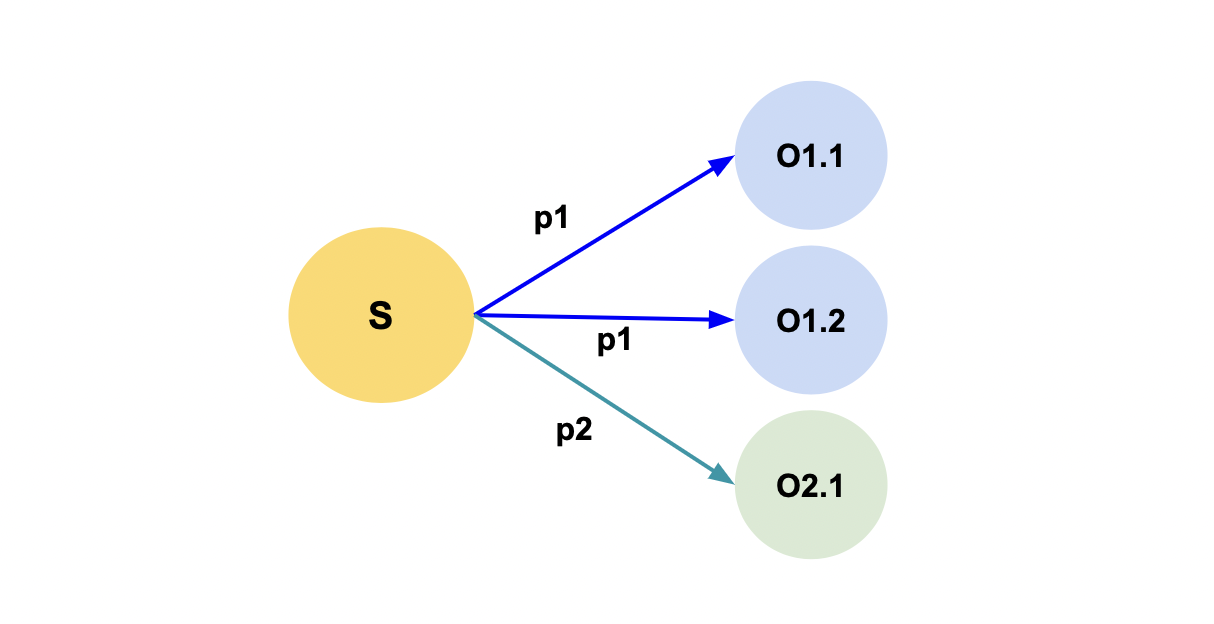
\includegraphics[scale=.3]{Wealth Type 1}
        \caption{Illustration of bag of properties and set of properties} \label{fig:wealth-type1}
    \end{subfigure}
    \hfill
    \begin{subfigure}[b]{0.3\textwidth}
        \centering
        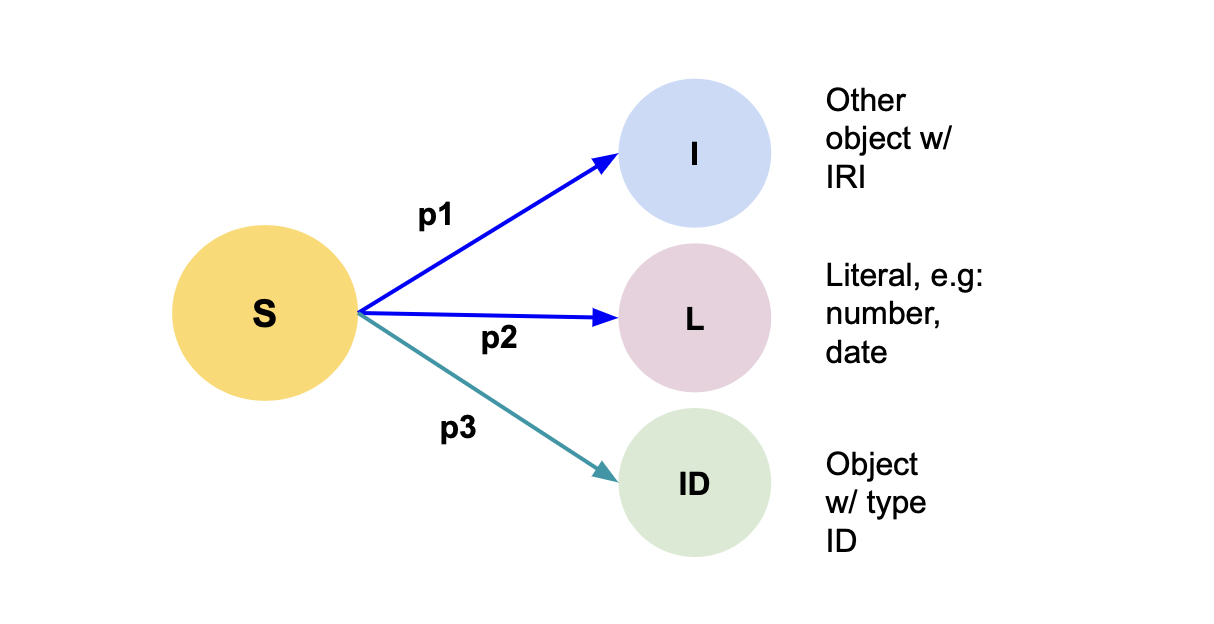
\includegraphics[scale=.3]{Wealth Type 2}
        \caption{Illustration of 3 types of property: object, literal, ID} \label{fig:wealth-type2}
    \end{subfigure}
    \hfill
    \begin{subfigure}[b]{0.3\textwidth}
        \centering
        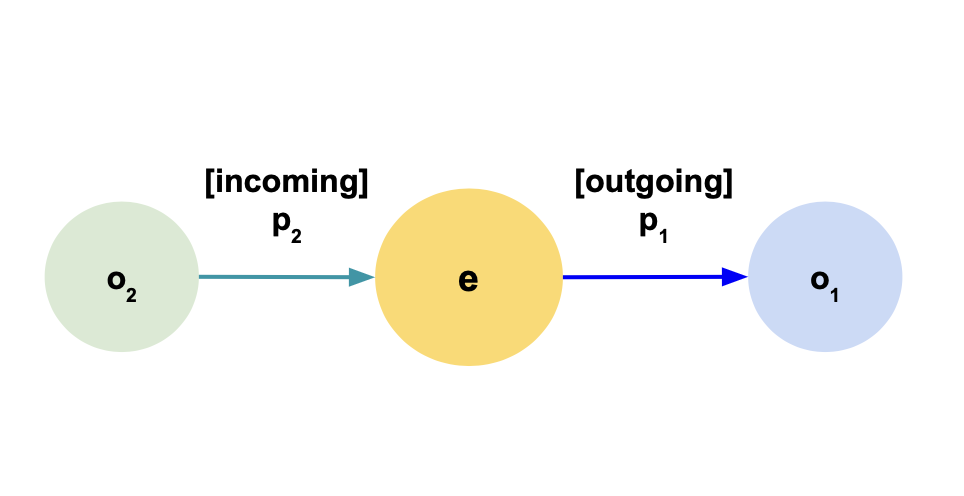
\includegraphics[scale=.3]{Wealth Type 3}
        \caption{Illustration of incoming link vs. outgoing link} \label{fig:wealth-type3}
    \end{subfigure}
    \caption{Three simple graphs} \label{fig:three graphs}
\end{figure}

\paragraph{Wealth based on the (non-)uniqueness of individual properties.}
The first aspect of knowledge wealth concerns how we regard the multiplicity or the (non-)uniqueness or the properties. Specifically, if an entity \(e\) has a property \(p_1\) that links it to a finite set of \(n\) distinct objects \(o_1\), \(o_2\), ..., \(o_n\), we may choose whether to account for the total number of objects associated with it (which is \(n\)), or to consider only the existence of \(p_1\). We refer to the former as the bag of properties, and the latter as the set of properties approach.

Under the bag of properties, an entity's knowledge wealth is defined as the cardinality of the set of triples in which it appears (either in the subject or object position, depending on the assumed link direction). For example, assuming an outgoing link direction, the triples \((e, p_1, o_1)\) and \((e, p_1, o_2)\) account for a wealth of 1 each, thus both have a total of 2. Formally, the knowledge wealth of an entity \(e\) under the bag of properties approach when no filtering is applied to the property type and using outgoing link direction, is denoted as \(W_{bag, *, [out]}(e,G)\) and is defined as:
% Similarly, if the incoming link direction is used, the triples \((s_1, p_1, e)\) and \((s_2, p_1, e)\) each contribute a wealth of 1, again totaling a wealth of 2. Formally, the knowledge wealth of an entity \(e\) under the bag of properties approach when no filtering is applied to the property type, is denoted as \(W_{bag, *, out}(e,G)\) when using outgoing link, and \(W_{bag, *, in}(e,G)\) when using incoming link, and is defined as:
\[
    W_{bag, *, [out]}(e,G) = |\{(p, o) | (e, p, o) \in G\}|
\]
% \[
%     W_{bag, *, in}(e,G) = |\{(s, p) | (s, p, e) \in G\}|
% \]

In the set of properties, knowledge wealth is measured by counting the number of distinct properties that describe the entity. By this way, we are capturing the variety of information about an entity. In contrast to bag of properties, in set of properties (with an assumption of outgoing link direction), \((e, p_1, o_1)\) and \((e, p_1, o_2)\) would be regarded as the "same" information because of the identical property \(p_1\), thus they only account for a total wealth of 1. Formally, the knowledge wealth of an entity \(e\) under the set of properties approach when no filtering is applied to the property type and using outgoing link direction, is denoted as \(W_{set, *, [out]}(e,G)\) and is defined as:
% Likewise, when using the incoming link direction, \((s_1, p_1, e)\) and \((s_2, p_1, e)\) are also treated as identical and collectively count as a single contribution to the entity's wealth. Formally, the knowledge wealth of an entity \(e\) under the set of properties approach when no filtering is applied to the property type, is denoted as \(W_{set, *, out}(e,G)\) when using outgoing link, and \(W_{set, *, in}(e,G)\) when using incoming link, and is defined as:
\[
    W_{set, *, [out]}(e,G) = |\{p | (e, p, o) \in G\}|
\]
% \[
%     W_{set, *, in}(e,G) = |\{(p) | (s, p, e) \in G\}|
% \]

% The first measure of the knowledge wealth of \(s\) is bag of properties---the cardinality of set of all triples that has \(s\) in their subject position. In this definition, the triples \((s, p_1, o_1)\) and \((s, p_1, o_2)\) account for a wealth of 1 each, thus both have a total of 2.

% Let \(N_{bag}(s,G)\) be a set that comprises all pair of predicate/property and object \((p,o)\) that is connected to \(s\). Then \(W_{bag}(s, G)\) is the cardinality of \(N_{bag}(s,G)\).
% \[
%     N_{bag}(s,G) = \{(p, o) | (s, p, o) \in G\}
% \]
% \[
%     W_{bag}(s,G) = |N_{bag}(s)|
% \]

% Another way of measuring the wealth is by counting the number of distinct properties describing the entity, or set of properties. By this way, we are capturing the variety of information about an entity. In contrast to bag of properties, in set of properties \((s, p_1, o_1)\) and \((s, p_1, o_2)\) would be regarded as the "same" information because of the identical property \(p_1\), thus they only account for a total wealth of 1. Let \(N_{set}(s,G)\) be a set that comprises all predicate/property \(p\) that is connected to \(s\). Then \(W_{set}(s, G)\) is the cardinality of \(N_{set}(s,G)\).
% \[
%     N_{set}(s, G) = \{p | \exists o, (s, p, o) \in G\}
% \]
% \[
%     W_{set}(s, G) = |N_{set}(s,G)|
% \]

% By the above definition, the wealth of entity \(s\) in \autoref{fig:wealth-type1} is 3 and 2, using bag of properties and set of properties respectively.

\paragraph{Wealth based on type of property.}
There are two main categories of properties in RDF: object properties, which link IRIs (on subject position) to IRIs (on object position), and datatype properties, which link IRIs (on subject position) to data literals (on object position)~\cite{w3crdf}. The idea of knowledge wealth based on property type is inspired by how human wealth is assessed across different types of possessions (e.g., real estate, vehicles, financial assets). Similarly, in knowledge graphs, property types can be seen as categories of informational assets that contribute to an entity's overall wealth.

This formulation allows us to evaluate not just how much information an entity has, but what kind of information it possesses. For instance, one entity may be rich in object links (e.g., affiliations or relationships to other entities), while another may be rich in literal facts (e.g., birth date, height). Segmenting wealth by property type thus provides a more nuanced view of an entity's informational profile.

Since each property \(p \in I\), we define the set of object properties as \(I_{objProp}\). Therefore, the knowledge wealth of an entity \(e\), based solely on object properties and using the bag of properties approach (assuming outgoing link direction) is defined as:
\[
    W_{bag,[obj],[out]}(e,G) = |\{(p,o) | ((e, p, o) \in G) \cap (p \in I_{objProp})\}|
\]

The handling for datatype properties is special. Among literal values, we see that there are two categories: pure literals, which are values that behave like constants or factual attributes (e.g., date of birth, height, population), and (external) IDs, which are string-based values that are used as identifier for the entity in external systems or databases (e.g., Freebase ID, IMDb ID). Based on this distinction, we define two corresponding subsets of datatype properties. The first one is \(I_{ltrProp}\) for the set of pure literals properties, and \(I_{idProp}\) for the set of IDs properties. Then, the knowledge wealth of an entity \(e\) under the bag of properties approach, using outgoing links, can be separately defined for each category as:
\[
    W_{bag,[ltr],[out]}(e,G) = |\{(p,o) | ((e, p, o) \in G) \cap (p \in I_{ltrProp})\}|
\]
\[
    W_{bag,[id],[out]}(e,G) = |\{(p,o) | ((e, p, o) \in G) \cap (p \in I_{idProp})\}|
\]

The sets \(I_{objProp}\), \(I_{ltrProp}\), and \(I_{idProp}\) are all mutually exclusive. We define their union as \(I_{Prop}\), the set of IRIs that function as properties (i.e., those used in the predicate position of RDF triples but not act as entity subjects or objects). Formally, this set is defined as:
\[
    I_{Prop} = (I_{objProp} \cup I_{ltrProp} \cup I_{idProp})
\]

When measuring the knowledge wealth of an entity \(e\), we may choose to filter by a specific property type or take a combination of them. For instance, in the previously defined measure \(W_{bag, *, [out]}(e,G)\), the assumption is that all property types are included (i.e., \(p \in I_{Prop}\)), while \(W_{bag, [obj, ltr], [out]}(e,G)\) includes only object and literal properties (i.e., \(p \in (I_{objProp} \cup I_{ltrProp})\))

% Object properties are other entities besides \(s\) that is connected with \(s\) through a property \(p\). Wealth of \(s\) using bag of properties with only considering the object properties is defined as:
% \[
%     W_{bag, object}(s, G) = |\{(p,o) | ((s, p, o) \in G) \cap (o \in I)\}|
% \]
% Literal properties are non-object properties that is connected with \(s\) through a property \(p\). Wealth of \(s\) using bag of properties with only considering the literal properties is defined as:
% \[
%     W_{bag, literal}(s, G) = |\{(p,o) | ((s, p, o) \in G) \cap (o \in L)\}|
% \]

% An external ID is a special type of string that is used to represent an entity in an external source. In Wikidata, an ID is identifiable by property type \textit{wikibase:ExternalId}. Just like any other property, an ID is connected with \(s\) through a property \(p\). Let  \(C_{ID,G}\) be a set comprising ID property in graph \(G\). Wealth of \(s\) using bag of properties with only considering the ID properties is defined as:
% \[
%     W_{bag, ID}(s, G) = |\{(p,o) | ((s, p, o) \in G) \cap (o \in L) \cap (o \in C_{ID,G})\}|
% \]

\paragraph{Wealth based on the direction of the link.}
In the previous definitions of knowledge wealth, we assumed that links originate from the entity \(e\); that is, \(e\) appears as the subject in the set of triples in graph \(G\). However, wealth can also be defined from the opposite perspective, where links point toward the entity. In this incoming link formulation, the properties contributing to the wealth of an entity \(e\) are derived from triples in which \(e\) appears as the object.

Under the bag of properties approach, in contrast to the outgoing link formulation where we count the pairs \(p, o\) from triples \(e, p, o\), in the incoming link case we count the pairs \(s, p\) from triples \(s, p, e\). In this definition, the triples \((s_1, p_1, e)\) and \((s_2, p_1, e)\) each contribute a wealth of 1 since the pairs \(s_1, p_1\) and \(s_2, p_1\) are treated as distinct. This results in a total wealth of 2 for the entity \(e\). Formally, the knowledge wealth of an entity \(e\) in this case is denoted as \(W_{bag, *, [in]}(e,G)\), and is defined as:

\[
    W_{bag, *, [in]}(e,G) = |\{(s, p) | (s, p, e) \in G\}|
\]

Likewise, under the set of properties approach and incoming link direction, the triples \((s_1, p_1, e)\) and \((s_2, p_1, e)\) are treated as identical since they share the same property \(p_1\), and collectively count as a single contribution to the entity's wealth. The corresponding formal definition for this case is denoted as \(W_{set, *, [in]}(e,G)\), and is defined as:

\[
    W_{set, *, [in]}(e,G) = |\{(p) | (s, p, e) \in G\}|
\]

It is important to note that, for the incoming link formulation, we always assume that \(p \in I_{objProp}\). This is because the object position in the triples is taken by the entity \(e\), and \(e \in I\) (\(e\) is not a literal/ID).

% In outgoing link type of wealth, the properties that are used in the wealth calculation of an entity \(s\) are those obtained from link with outwards direction from that particular entity \(s\); that is where \(s\) appears to be the subject in the set of triples in graph \(G\). All types of wealth defined before use the notion of outgoing link.

% In incoming link type of wealth, the properties that are used in the wealth calculation of an entity \(s\) are those obtained from link with inwards direction to that particular entity \(s\); that is where \(s\) appears to be the object in the set of triples in graph \(G\). To illustrate, let \(N_{bag}(s)\) be a set that comprises all pair of object and predicate/property \((o,p)\) that is connected to \(s\) in incoming direction to \(s\) i.e., \(N_{bag}(s)\) = \(\{(o, p) | (o, p, s) \in G\}\). Then the wealth of \(s\) using bag of properties and the view of incoming link is notated as \(W_{bag, incoming}(s, G)\), and equal to the cardinality of \(N_{bag}(s)\).
% \[
%     N_{bag, incoming}(s, G) = \{(o,p) | (o, p, s) \in G\}
% \]
% \[
%     W_{bag, incoming}(s, G) = |N_{bag, incoming}(s, G)|
% \]

% Looking at in \autoref{fig:wealth-type3}, the wealth of entity \(s\) is 1 using outgoing link, which is from the triple \((s, p_1, o1)\). Its wealth is also 1 and using incoming link, which comes from the triple \((o2, p_2, s)\).

% Each definition above can be used simultaneously. For example, the wealth of entity \(s\) using set of properties, calculating object and data but not ID properties, and using the direction of outgoing link is denoted by \(W_{set, outgoing, (object \cup data) \cap ID^\complement}(s, G) = |N_{set, outgoing, (object \cup data) \cap ID^\complement}(s, G)|\) with \(N_{set, outgoing, (object \cup data) \cap ID^\complement}(s, G) = \{p | \exists o, (s, p, o) \in G, \cap (o \in ((I \cup L) \cap C_{ID,G}^\complement))\}\).

\begin{center}
    \scriptsize
    \makebox[\linewidth]{
    \begin{threeparttable}
    \captionsetup{font=small}
    \caption{Wealth Formal Definitions}
    \label{tab:wealth-formal-definition}
    \begin{tabular}{|c | c c c c c c |} 
    
    \toprule
        No & Formal Notation & Multiplicity & \CellWithForceBreak{Property \\ Type} & \CellWithForceBreak{Link \\ Direction} & Formal Definition & Notes \\ [0.5ex] 
    \midrule
        1 & $W_{bag,*,[out]}(e,G)$ & Bag & * & Out & $|\{(p, o) | (e, p, o) \in G\}|$ & \\
        2 & $W_{bag,[obj],[out]}(e,G)$ & Bag & Object & Out & $|\{(p,o) | ((e, p, o) \in G) \cap (p \in I_{objProp})\}|$ & \\
        3 & $W_{bag,[ltr],[out]}(e,G)$ & Bag & Literal & Out & $|\{(p,o) | ((e, p, o) \in G) \cap (p \in I_{ltrProp})\}|$ & \\
        4 & $W_{bag,[id],[out]}(e,G)$ & Bag & ID & Out & $|\{(p,o) | ((e, p, o) \in G) \cap (p \in I_{idProp})\}|$ & \\
        5 & $W_{bag,[obj, ltr],[out]}(e,G)$ & Bag & Object, literal & Out & $|\{(p,o) | ((e, p, o) \in G) \cap (p \in (I_{objProp} \cup I_{ltrProp}))\}|$ & \\
        6 & $W_{bag,[obj, id],[out]}(e,G)$ & Bag & Object, ID & Out & $|\{(p,o) | ((e, p, o) \in G) \cap (p \in (I_{objProp} \cup I_{idProp}))\}|$ & \\
        7 & $W_{bag,[ltr, id],[out]}(e,G)$ & Bag & Literal, ID & Out & $|\{(p,o) | ((e, p, o) \in G) \cap (p \in (I_{ltrProp} \cup I_{idProp}))\}|$ & \\

        8 & $W_{bag,*,[in]}(e,G)$ & Bag & * & In & $|\{(s, p) | (s, p, e) \in G\}|$ & \\
        9 & $W_{bag,[obj],[in]}(e,G)$ & Bag & Object & In & $|\{(s,p) | ((s, p, e) \in G) \cap (p \in I_{objProp})\}|$ & \\
        10 & $W_{bag,[ltr],[in]}(e,G)$ & Bag & Literal & In & $|\emptyset| = 0$ & \CellWithForceBreak{$p \in I_{objProp}$ \\ because $e \in I$} \\
        11 & $W_{bag,[id],[in]}(e,G)$ & Bag & ID & In & $|\emptyset| = 0$ & \CellWithForceBreak{$p \in I_{objProp}$ \\ because $e \in I$} \\
        12 & $W_{bag,[obj, ltr],[in]}(e,G)$ & Bag & Object, literal & In & $|\{(s,p) | ((s, p, e) \in G) \cap (p \in I_{objProp})\}|$ & \CellWithForceBreak{$p \in I_{objProp}$ \\ because $e \in I$} \\
        13 & $W_{bag,[obj, id],[in]}(e,G)$ & Bag & Object, ID & In & $|\{(s,p) | ((s, p, e) \in G) \cap (p \in I_{objProp})\}|$ & \CellWithForceBreak{$p \in I_{objProp}$ \\ because $e \in I$} \\
        14 & $W_{bag,[ltr, id],[in]}(e,G)$ & Bag & Literal, ID & In & $|\emptyset| = 0$ & \CellWithForceBreak{$p \in I_{objProp}$ \\ because $e \in I$} \\

        15 & $W_{bag,*,*}(e,G)$ & Bag & * & * & $|\{(p, o) | (e, p, o) \in G\}| + |\{(s, p) | (s, p, e) \in G\}|$ & \CellWithForceBreak{Aggregation of \\ \#1 and \#8} \\
        16 & $W_{bag,[obj],*}(e,G)$ & Bag & Object & * &  \CellWithForceBreak{$|\{(p,o) | ((e, p, o) \in G) \cap (p \in I_{objProp})\}|$ \\ $ + |\{(s,p) | ((s, p, e) \in G) \cap (p \in I_{objProp})\}|$} & \CellWithForceBreak{Aggregation of \\ \#2 and \#9} \\
        17 & $W_{bag,[ltr],*}(e,G)$ & Bag & Literal & * & $|\{(p,o) | ((e, p, o) \in G) \cap (p \in I_{ltrProp})\}|$ & \CellWithForceBreak{Aggregation of \\ \#3 and \#10} \\
        18 & $W_{bag,[id],*}(e,G)$ & Bag & ID & * & $|\{(p,o) | ((e, p, o) \in G) \cap (p \in I_{idProp})\}|$ & \CellWithForceBreak{Aggregation of \\ \#4 and \#11} \\
        19 & $W_{bag,[obj, ltr],*}(e,G)$ & Bag & Object, literal & * & \CellWithForceBreak{$|\{(p,o) | ((e, p, o) \in G) \cap (p \in (I_{objProp} \cup I_{ltrProp}))\}|$  \\ $ + |\{(s,p) | ((s, p, e) \in G) \cap (p \in I_{objProp})\}|$} & \CellWithForceBreak{Aggregation of \\ \#5 and \#12} \\
        20 & $W_{bag,[obj, id],*}(e,G)$ & Bag & Object, ID & * & \CellWithForceBreak{$|\{(p,o) | ((e, p, o) \in G) \cap (p \in (I_{objProp} \cup I_{idProp}))\}|$ \\ $ + |\{(s,p) | ((s, p, e) \in G) \cap (p \in I_{objProp})\}|$} & \CellWithForceBreak{Aggregation of \\ \#6 and \#13} \\
        21 & $W_{bag,[ltr, id],*}(e,G)$ & Bag & Literal, ID & * & $|\{(p,o) | ((e, p, o) \in G) \cap (p \in (I_{ltrProp} \cup I_{idProp}))\}|$ & \CellWithForceBreak{Aggregation of \\ \#7 and \#14} \\

        22 & $W_{set,*,[out]}(e,G)$ & Set & * & Out & $|\{p | (e, p, o) \in G\}|$ & \\
        23 & $W_{set,[obj],[out]}(e,G)$ & Set & Object & Out & $|\{p | ((e, p, o) \in G) \cap (p \in I_{objProp})\}|$ & \\
        24 & $W_{set,[ltr],[out]}(e,G)$ & Set & Literal & Out & $|\{p | ((e, p, o) \in G) \cap (p \in I_{ltrProp})\}|$ & \\
        25 & $W_{set,[id],[out]}(e,G)$ & Set & ID & Out & $|\{p | ((e, p, o) \in G) \cap (p \in I_{idProp})\}|$ & \\
        26 & $W_{set,[obj, ltr],[out]}(e,G)$ & Set & Object, literal & Out & $|\{p | ((e, p, o) \in G) \cap (p \in (I_{objProp} \cup I_{ltrProp}))\}|$ & \\
        27 & $W_{set,[obj, id],[out]}(e,G)$ & Set & Object, ID & Out & $|\{p | ((e, p, o) \in G) \cap (p \in (I_{objProp} \cup I_{idProp}))\}|$ & \\
        28 & $W_{set,[ltr, id],[out]}(e,G)$ & Set & Literal, ID & Out & $|\{p | ((e, p, o) \in G) \cap (p \in (I_{ltrProp} \cup I_{idProp}))\}|$ & \\
        29 & $W_{set,*,[in]}(e,G)$ & Set & * & In & $|\{p | (s, p, e) \in G\}|$ & \\
        30 & $W_{set,[obj],[in]}(e,G)$ & Set & Object & In & $|\{p | ((s, p, e) \in G) \cap (p \in I_{objProp})\}|$ & \\
        31 & $W_{set,[ltr],[in]}(e,G)$ & Set & Literal & In & $|\emptyset| = 0$ & \CellWithForceBreak{$p \in I_{objProp}$ \\ because $e \in I$} \\
        32 & $W_{set,[id],[in]}(e,G)$ & Set & ID & In & $|\emptyset| = 0$ & \CellWithForceBreak{$p \in I_{objProp}$ \\ because $e \in I$} \\
        33 & $W_{set,[obj, ltr],[in]}(e,G)$ & Set & Object, literal & In & $|\{p | ((s, p, e) \in G) \cap (p \in I_{objProp})\}|$ & \CellWithForceBreak{$p \in I_{objProp}$ \\ because $e \in I$} \\
        34 & $W_{set,[obj, id],[in]}(e,G)$ & Set & Object, ID & In & $|\{p | ((s, p, e) \in G) \cap (p \in I_{objProp})\}|$ & \CellWithForceBreak{$p \in I_{objProp}$ \\ because $e \in I$} \\
        35 & $W_{set,[ltr, id],[in]}(e,G)$ & Set & Literal, ID & In & $|\emptyset| = 0$ & \CellWithForceBreak{$p \in I_{objProp}$ \\ because $e \in I$} \\
        36 & $W_{set,*,*}(e,G)$ & Set & * & * & $|\{p | (e, p, o) \in G\}| + |\{p | (s, p, e) \in G\}|$ & \CellWithForceBreak{Aggregation of \\ \#22 and \#29}\\
        37 & $W_{set,[obj],[out]}(e,G)$ & Set & Object & Out & \CellWithForceBreak{$|\{p | ((e, p, o) \in G) \cap (p \in I_{objProp})\}|$ \\ $+ |\{p | ((s, p, e) \in G) \cap (p \in I_{objProp})\}|$} & \CellWithForceBreak{Aggregation of \\ \#23 and \#30}\\
        38 & $W_{set,[ltr],[out]}(e,G)$ & Set & Literal & Out & $|\{p | ((e, p, o) \in G) \cap (p \in I_{ltrProp})\}|$ & \CellWithForceBreak{Aggregation of \\ \#24 and \#31}\\
        39 & $W_{set,[id],[out]}(e,G)$ & Set & ID & Out & $|\{p | ((e, p, o) \in G) \cap (p \in I_{idProp})\}|$ & \CellWithForceBreak{Aggregation of \\ \#25 and \#32}\\
        40 & $W_{set,[obj, ltr],[out]}(e,G)$ & Set & Object, literal & Out & \CellWithForceBreak{$|\{p | ((e, p, o) \in G) \cap (p \in (I_{objProp} \cup I_{ltrProp}))\}|$ \\ $+ |\{p | ((s, p, e) \in G) \cap (p \in I_{objProp})\}|$} & \CellWithForceBreak{Aggregation of \\ \#26 and \#33}\\
        41 & $W_{set,[obj, id],[out]}(e,G)$ & Set & Object, ID & Out & \CellWithForceBreak{$|\{p | ((e, p, o) \in G) \cap (p \in (I_{objProp} \cup I_{idProp}))\}|$ \\ $+ |\{p | ((s, p, e) \in G) \cap (p \in I_{objProp})\}|$} & \CellWithForceBreak{Aggregation of \\ \#27 and \#34}\\
        42 & $W_{set,[ltr, id],[out]}(e,G)$ & Set & Literal, ID & Out & $|\{p | ((e, p, o) \in G) \cap (p \in (I_{ltrProp} \cup I_{idProp}))\}|$ & \CellWithForceBreak{Aggregation of \\ \#28 and \#35}\\

    \bottomrule
    \end{tabular}
    \begin{tablenotes}
        \scriptsize
        \item{This table summarizes the 30 formal definitions of knowledge wealth used in this study. Each row represents a variant of wealth based on three key dimensions: (1) multiplicity: bag or set; (2) property type: object, literal, ID, or any of their combinations; and (3) link direction: in, out, or any of their combinations. In the notation used in the table, \(G\) denotes the RDF knowledge graph, \(e\) is an entity (instance) in that graph. Each triple in the graph is composed of a subject \(s\), a property \(p\), and an object \(o\). \(I\) the set of all IRIs in the graph, \(I_objProp\) is the set of IRIs used as object properties, \(I_ltrProp\) is the set of IRIs used as pure literal properties, and \(I_idProp\) is the set of IRIs used as identifier properties. \(I_{Prop} = (I_{objProp} \cup I_{ltrProp} \cup I_{idProp})\) is the set of all valid property IRIs.}
    \end{tablenotes}
    \end{threeparttable}
    }
\end{center}

\subsubsection{Class-Level Wealth}
In this study, we re-use the class model defined by Ramadizsa et al.~\cite{RamadizsaDNR23}. A class is a group of entities that are the subject of the study. \textit{Human}, \textit{film}, and \textit{taxon} are some examples of class. In general, entity \(s\) is an instance of class \(C\) is expressed by the triple (\(s\), \textit{instanceOf}, \(C\)) or (\(s\), \textit{type}, \(C\)). We can get a more narrow class inside the defined class by specifying additional conditions, each consisting of a particular property and value associated with it. Example of such conditions for human class is \textit{gender} with associated value \textit{male}, while example for a country would be \textit{continent} with value \textit{Asia}. For instance, the class of human with gender male that lived during English Renaissance is queried using (\(?s\), \{(\(?s\), \textit{instanceOf}, \textit{human}), (\(?s\), \textit{gender}, \textit{male}), (\(?s\), \textit{timePeriod}, \textit{EnglishRenaissance})\}).

Let \(C\) be a class that consists of \(m\) distinct entities \(s_1\), \(s_2\), ... \(s_m\) in graph \(G\). We define \(T_C\) a multiset consists of the wealth of each entity of \(C\), i.e., 
\[
    T_{C,G} = \{W(s_1), G, W(s_2, G), W(s_3, G), ..., W(s_m, G)\}
\] 
We denote the overall wealth of class \(C\) as \(\mathcal{W}(C)\). It can be quantified using its constituent entities and be expressed as a function of \(T_C\), denoted as \(f(T_C)\), where \(f\) may represent statistical summaries such as the cardinality (i.e., entity count), sum, mean, median, mode, or percentile of its entities's wealth.
\[
    \mathcal{W}(C,G) = f(T_{C,G})
\]
As an example, consider a class \(C\) consisting of of 4 entities  \(s_1\), \(s_2\), \(s_3\), and \(s_4\) from \autoref{fig:wealth-weighted}. If we use cardinality as the function \(f\), then \(\mathcal{W}(C) = 4\), corresponding to the number of entities it contains.

It is important to note that not all statistical functions are suitable for this purpose. The previously mentioned functions provide interpretable measures of central tendency or overall volume, thus they are considered valid to be used as \(f\) to represent the level of wealth of a class. On the contrary, inequality metrics such as the Gini coefficient or standard deviation are designed to capture distributional imbalance rather than the actual level of wealth, and therefore are not appropriate as definitions of \(\mathcal{W}(C)\), which aims to describe how rich a class is, and not how unequal the wealth distribution is within it.